\section{Experiment}
First, we formulate a constrained problem by searching the optimal stacking
sequence of cross-ply laminate under in-plane loading whose strength ratio is
not less than 2.  Each lamina dimensions $1000 \times 1000 \times 0.165 mm^3$
is adopted in this experiment, each graphite/epoxy,  and glass/epoxy layer is
assumed to cost 2.5 and 1 monetary units, respectively. The other material
properties are shown in Table \ref{tab:mat}. 


\subsection{Problem formulation}

In the present experiment, the optimal composite sequences, and the number of
layers for a targeted strength ratio under in-plane loading conditions are
investigated.  The aim is to minimize the mass of a laminate composite for a
targeted strength ratio based on the Tsai-wu failure theory. The design
variables are the ply angles and the number of layers.  Ply orientation
restricted to a discrete set of angles ($0, \text{ and } 90 \text{ degrees} $).
The problem can be formulated as the following equation

Find: $\{\theta_k, n\}$ $\theta_k \in \{ 0,90\}$

Minimize: weight

Subject to: strength ratio


\subsection{GA Operation}

\begin{figure}[!htb]
\setlength{\fboxsep}{0pt}%
\setlength{\fboxrule}{0pt}%
\begin{center}
\resizebox{.95\linewidth}{!}{
		\begin{tikzpicture}
		\tikzstyle{rec} = [rectangle, minimum width=0.8cm,minimum height=0.6cm, text
		centered, draw=black]
			\node (gene11) [rec] {90};
			\node (gene2) [rec] at ($(gene11.east)+(0.4cm,0)$)  {90};
			\node (gene3) [rec] at ($(gene2.east)+(0.4cm,0)$)  {0};
			\node (gene4) [rec] at ($(gene3.east)+(0.4cm,0)$)  {0};
			\node (gene5) [rec] at ($(gene4.east)+(0.4cm,0)$)  {0};
			\node (gene6) [rec] at ($(gene5.east)+(0.4cm,0)$)  {90};
			\node (gene7) [rec] at ($(gene6.east)+(0.4cm,0)$)  {90};
			\node (gene8) [rec] at ($(gene7.east)+(0.4cm,0)$)  {90};
			\node (gene9) [rec] at ($(gene8.east)+(0.4cm,0)$)  {90};
			\node (last) [rec] at ($(gene9.east)+(0.4cm,0)$)  {90};
			\node[text width=1cm] at ($(gene11.west)+(-0.3cm,0)$) {$P_1$:};
			\node (gene1) [rec] at ($(gene11.east)+(-0.4cm,-0.8cm)$) {0};
			\node (gene2) [rec] at ($(gene1.east)+(0.4cm,0)$)  {0};
			\node (gene3) [rec] at ($(gene2.east)+(0.4cm,0)$)  {90};
			\node (gene4) [rec] at ($(gene3.east)+(0.4cm,0)$)  {90};
			\node (gene5) [rec] at ($(gene4.east)+(0.4cm,0)$)  {90};
			\node (gene6) [rec] at ($(gene5.east)+(0.4cm,0)$)  {0};
			\node (gene7) [rec] at ($(gene6.east)+(0.4cm,0)$)  {0};
			\node (gene8) [rec] at ($(gene7.east)+(0.4cm,0)$)  {90};
			\node (gene9) [rec] at ($(gene8.east)+(0.4cm,0)$)  {0};
			\node (gene10) [rec] at ($(gene9.east)+(0.4cm,0)$)  {0};
			\node[text width=1cm] at ($(gene1.west)+(-0.3cm,0)$) {$P_2$:};
			\draw[-,white] ($(gene10.north)$)-- ++(0,-1.5cm);
			\node (label1) at ($(gene5.south)+(0cm,-0.5cm)$) {(a): Parents $P_1$ and $P_2$};
		\end{tikzpicture}
}

% offspring
\resizebox{.95\linewidth}{!}{
		\begin{tikzpicture}
			\tikzstyle{rec} = [rectangle, minimum width=0.8cm,minimum height=0.6cm, text
			centered, draw=black]
			\node (gene11) [rec] {90};
			\node (gene2) [rec] at ($(gene11.east)+(0.4cm,0)$) {90};
			\node (gene3) [rec] at ($(gene2.east)+(0.4cm,0)$)  {0};
			\node (gene4) [rec] at ($(gene3.east)+(0.4cm,0)$)  {0};
			\node (gene5) [rec] at ($(gene4.east)+(0.4cm,0)$)  {0};
			\node (gene6) [rec] at ($(gene5.east)+(0.4cm,0)$)  {0};
			\node (gene7) [rec] at ($(gene6.east)+(0.4cm,0)$)  {0};
			\node (gene8) [rec] at ($(gene7.east)+(0.4cm,0)$)  {90};
			\node (gene9) [rec] at ($(gene8.east)+(0.4cm,0)$)  {0};
			\node (last) [rec] at ($(gene9.east)+(0.4cm,0)$)  {0};
			\node[text width=1cm] at ($(gene11.west)+(-0.3cm,0)$) {$O_1$:};
			\node (gene1) [rec] at ($(gene11.east)+(-0.4cm,-0.8cm)$) {0};
			\node (gene2) [rec] at ($(gene1.east)+(0.4cm,0)$)  {0};
			\node (gene3) [rec] at ($(gene2.east)+(0.4cm,0)$)  {90};
			\node (gene4) [rec] at ($(gene3.east)+(0.4cm,0)$)  {90};
			\node (gene5) [rec] at ($(gene4.east)+(0.4cm,0)$)  {90};
			\node (gene6) [rec] at ($(gene5.east)+(0.4cm,0)$)  {90};
			\node (gene7) [rec] at ($(gene6.east)+(0.4cm,0)$)  {90};
			\node (gene8) [rec] at ($(gene7.east)+(0.4cm,0)$)  {90};
			\node (gene9) [rec] at ($(gene8.east)+(0.4cm,0)$)  {90};
			\node (gene10) [rec] at ($(gene9.east)+(0.4cm,0)$)  {90};
			\node[text width=1cm] at ($(gene1.west)+(-0.3cm,0)$) {$O_2$:};
			\draw[-,white] ($(gene10.north)$)-- ++(0,-1.5cm);
			\node (label1) at ($(gene5.south)+(0cm,-0.5cm)$) {(b): Offspring $O_1$ and $O_2$};
		\end{tikzpicture}
}

%mutation
\resizebox{.95\linewidth}{!}{
	\begin{tikzpicture}
	\tikzstyle{rec} = [rectangle, minimum width=0.8cm,minimum height=0.6cm, text
	centered, draw=black]
		\tikzstyle{rec} = [rectangle, minimum width=0.8cm,minimum height=0.6cm, text
		centered, draw=black]
		%\draw[help lines](-3,-3) grid (4,4);
		\node (gene11) [rec] {90};
		\node (gene2) [rec] at ($(gene11.east)+(0.4cm,0)$)  {90};
		\node (gene3) [rec] at ($(gene2.east)+(0.4cm,0)$)  {90};
		\node (gene4) [rec] at ($(gene3.east)+(0.4cm,0)$)  {$\cdots$};
		\node (gene5) [rec] at ($(gene4.east)+(0.4cm,0)$)  {90};
		\node (gene6) [rec] at ($(gene5.east)+(0.4cm,0)$)  {90};
		\node (gene7) [rec] at ($(gene6.east)+(0.4cm,0)$)  {0};
		\node (gene8) [rec] at ($(gene7.east)+(0.4cm,0)$)  {$\cdots$};
		\node (gene9) [rec] at ($(gene8.east)+(0.4cm,0)$)  {0};
		\node (last) [rec] at ($(gene9.east)+(0.4cm,0)$)  {0};
		\draw[<->,thick] (gene11.south) .. controls +(1.8,-0.4) .. (gene6.south)
			node[pos=0.5] {10} ;
		\draw[<->,thick] (gene7.south) .. controls +(1.3,-0.4) .. (last.south)
			node[pos=0.5] {9};
		\node[text width=1cm] at ($(gene11.west)+(-0.3cm,0)$) {$O_1$:};

		\node (label1) at ($(gene5.south)+(0cm,-0.8cm)$) {(c): Offspring $O_1$ after
			lenght mutation};

		\node (gene1) [rec] at ($(gene11.east)+(-0.4cm,-1.8cm)$) {90};
		\node (gene2) [rec] at ($(gene1.east)+(0.4cm,0)$)  {90};
		\node (gene3) [rec] at ($(gene2.east)+(0.4cm,0)$)  {90};
		\node (gene4) [rec] at ($(gene3.east)+(0.4cm,0)$)  {$\cdots$};
		\node (gene5) [rec] at ($(gene4.east)+(0.4cm,0)$)  {90};
		\node (gene6) [rec] at ($(gene5.east)+(0.4cm,0)$)  {0};
		\node (gene7) [rec] at ($(gene6.east)+(0.4cm,0)$)  {0};
		\node (gene8) [rec] at ($(gene7.east)+(0.4cm,0)$)  {$\cdots$};
		\node (gene9) [rec] at ($(gene8.east)+(0.4cm,0)$)  {0};
		\node (last) [rec] at ($(gene9.east)+(0.4cm,0)$)  {0};
		\node[text width=1cm] at ($(gene11.west)+(-0.3cm,0)$) {$O_1$:};
		\draw[-,white] ($(gene10.north)$)-- ++(0,-1.5cm);
		\node (label1) at ($(gene5.south)+(0cm,-0.5cm)$) {(d): Offspring $O_1$ 
			 after angle mutation};
	\end{tikzpicture}
}
\end{center}
\caption{Examples of crossover, length mutation, angle  mutation operator for proposed GA.}
\label{GA:operator}
\end{figure}


In the present study, floating encoding is adopted to represent a solution for
the lay-up design of cross-ply laminate, figure \ref{GA:operator}(a) shows two
parents $P_1$ and $P_2$ which represent two cross-ply laminates, the
corresponding laminates lay-ups are $[0_3/90_7]$ and $[0_6/90_4]$,
respectively; figure \ref{GA:operator}(b) shows two offspring of parents $P_1$
and $P_2$ which are consist of half of each parent's chromosome; figure
\ref{GA:operator}(c) and \ref{GA:operator}(d) display the offspring after
length and angle mutation, respectively.

For the chromosome length mutation, calculate the chromosome's strength ratio
based on its sequence, if its strength ratio is less than the threshold, then
increase its length; otherwise, reduce it. We introduce the term length
mutation coefficient to control the length mutation.  As shown in figure
\ref{GA:operator}(b), the strength ratio of $O_1$ chromosome is 0.0854, and the
strength ratio threshold is five. Suppose the length mutation coefficient takes
two, then the corresponding increase length is the multiplication result of
length mutation coefficient and the difference between current strength ratio
and the threshold: the result is $5\times(2-0.0854)$, round this number to its
closest integer, which is 9. So the length of offspring $O_1$ changes from 10
to 19 after length mutation.  For the angle mutation, randomly swap the gene
from 0 to 90 in the chromosome, or the otherwise.


\subsection{GA Parameters}
Table \ref{tab:ga} shows related GA parameters: the population is 40, and 50
percent is as the mating pool, so the parent population is 20; as
shown in figure \ref{fig:percentage}, the percentage of active individuals from
the active group, potential individuals from the potential group, and proper
individuals from the proper group are 0.3, 0.3, and 0.4, which means the
corresponding number of these three types of individuals are 6, 6, and 8,
respectively.

\begin{figure}[!htb]
	\centering
	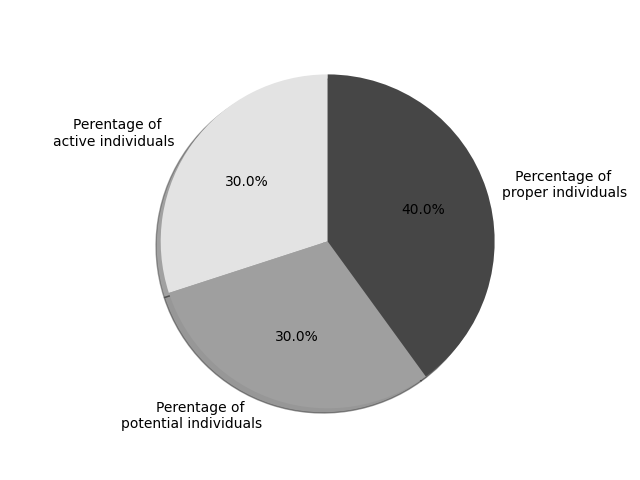
\includegraphics[width=\linewidth]{fig/percentage_of_groups}
	\caption{Percentage of active individuals from active group, potential
	  individuals from potential group, and proper individuals from proper group
	 in parent population.}
	 \label{fig:percentage}
\end{figure}

\begin{table}[!htb]
\centering
\caption{Parameters of proposed GA model.}
\begin{adjustbox}{width=0.45\textwidth}
\label{tab:ga}
\begin{tabular}{lc}
\toprule
Parameter								&  Value  \\
\midrule
Population                              & 40        \\
Initial length range					& [3-15]    \\
Encoding								& Integer   \\
Percentage of parent                    & 0.5   \\
Percentage of active group				& 0.3   \\
Percentage of potential group			& 0.3   \\
Percentage of proper group				& 0.4   \\
Selection strategy for  active group	& Ranking   \\
Selection strategy for potential group	& Ranking   \\
Selection strategy for proper group	    & Ranking   \\
Crossover strategy			    		& One-point \\
Mutation strategy			    		& Mass mutation \\
Length mutation coefficient             & 5 \\
Angle mutation rate                     & 0.1 \\
\bottomrule
\end{tabular}
\end{adjustbox}
\end{table}


